\section*{Appendix}

\begin{frame}{Further Improvements of Mining Methods}
	\begin{itemize}
		\item \textbf{AFOPT} (Liu et al., KDD'03)
		      \begin{itemize}
			      \item A "push-right" method for mining condensed frequent-pattern
			            (CFP) tree.
		      \end{itemize}
		\item \textbf{Carpenter} (Pan et al., KDD'03)
		      \begin{itemize}
			      \item Mine datasets with small rows but numerous columns.
			      \item Construct a row-enumeration tree for efficient mining.
		      \end{itemize}
		\item \textbf{FP-growth+} (Grahne \& Zhu, FIMI'03)
		      \begin{itemize}
			      \item Efficiently using prefix-trees in mining frequent itemsets.
		      \end{itemize}
		\item \textbf{TD-Close} (Liu et al., SDM'06)
	\end{itemize}
\end{frame}

\begin{frame}{Extension of Pattern-growth Mining Methodology}
	\begin{itemize}
		\item \textbf{Mining closed frequent itemsets and max-patterns.}
		      \begin{itemize}
			      \item CLOSET (DMKD'00), FPclose, and FPMax (Grahne \& Zhu, FIMI'03)
		      \end{itemize}
		\item \textbf{Mining sequential patterns.}
		      \begin{itemize}
			      \item PrefixSpan (ICDE'01), CloSpan (SDM'03), BIDE (ICDE'04)
		      \end{itemize}
		\item \textbf{Mining graph patterns.}
		      \begin{itemize}
			      \item gSpan (ICDM'02), CloseGraph (KDD'03)
		      \end{itemize}
		\item \textbf{Constraint-based mining of frequent patterns.}
		      \begin{itemize}
			      \item Convertible constraints (ICDE'01), gPrune (PAKDD'03)
		      \end{itemize}
		\item \textbf{Computing iceberg data cubes with complex measures.}
		      \begin{itemize}
			      \item H-tree, H-cubing, and Star-cubing (SIGMOD'01, VLDB'03)
		      \end{itemize}
		\item \textbf{Pattern-growth-based clustering.}
		      \begin{itemize}
			      \item MaPle (Pei et al., ICDM'03)
		      \end{itemize}
		\item \textbf{Pattern-growth-based classification.}
		      \begin{itemize}
			      \item Mining frequent and discriminative patterns (Cheng et al.,
			            ICDE'07)
		      \end{itemize}
	\end{itemize}
\end{frame}

\begin{frame}{Visualization of Association Rules (I)}
	\centering
	\scalebox{0.9}{
		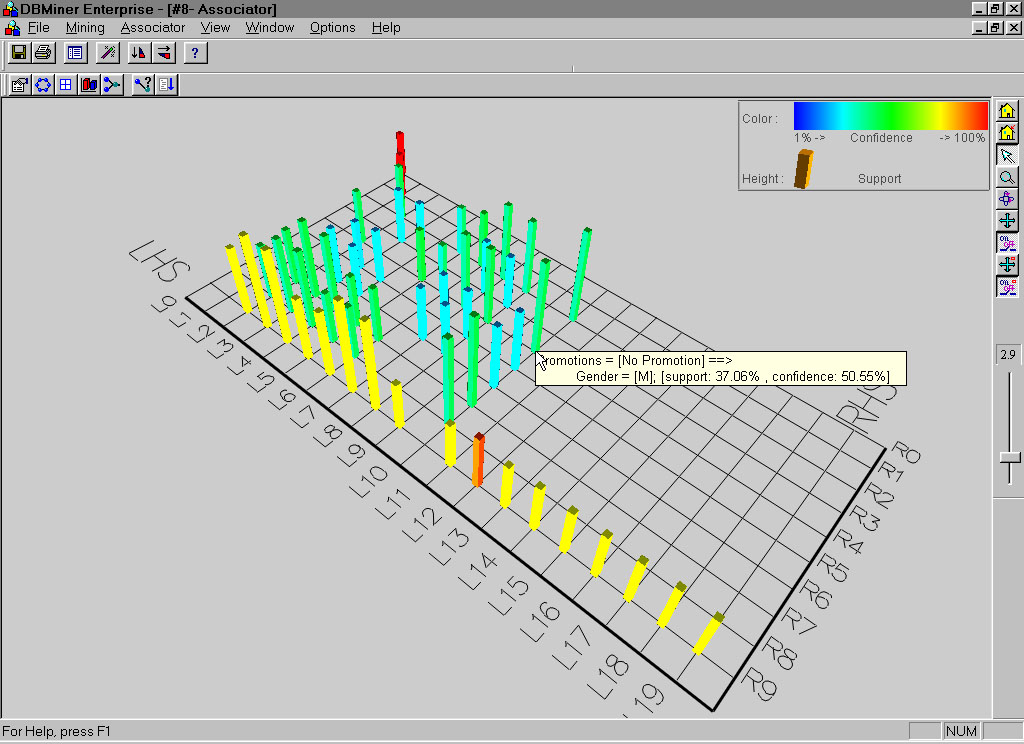
\includegraphics[width=0.6\textwidth]{img/assoc_rules1.jpg}
	}
	% In fact, these two illustrations are still the best visualization of assocaition rules I could find. Alternatives would % be the visualizations from e.g. this Jupyter Notebook experiment:
	% https://goldinlocks.github.io/Market-Basket-Analysis-in-Python/.
	% It may also be useful to revisit these graphics once we have completed our exercise sheets.
\end{frame}

\begin{frame}{Visualization of Association Rules (II)}
	\centering
	\scalebox{0.9}{
		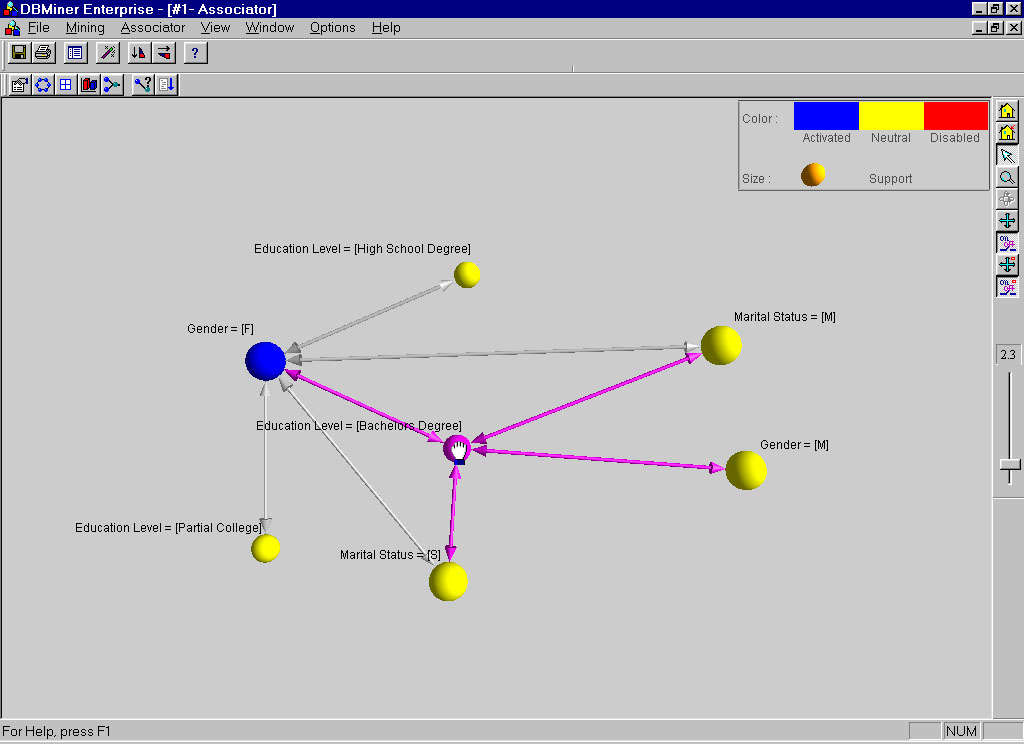
\includegraphics[width=0.6\textwidth]{img/assoc_rules2.jpg}
	}
\end{frame}
